\documentclass[../../main.tex]{subfiles}

\begin{document}
    Im letzten Abschnitt widmen wir uns dem Hauptziel des Experiments, der Kartierung der Milchstraße. Hierzu rastern wir, den bereits aufgenommenen Messdaten anhängend, in einem neuen Winkelabstand von $\SI{10}{\degree}$ ab $\SI{90}{\degree}$ galaktischer Länge bis $\SI{210}{\degree}$ inklusive $\SI{215}{\degree}$ und verfolgen damit die Bahn $s_*(t) = \delta t\cdot t + \SI{90}{\degree}$. Die Messung erfolgt weiterhin im \emph{switched mode}.
    
    Zunächst betrachten wir den erhaltenen Datensatz für sich und rechnen die Peakpunkte in Ortsangaben einer polaren Karte um. Hierzu verwenden wir die Radiusfunktion 
    \[
        R(V_r,l):= \frac{R_\odot\cdot V_\odot\cdot\sin(l)}{V_\odot\cdot\sin(l) + V_r}.
    \]
    Mithilfe einer geometrischen Identität $R(V_r,l)^2 = R_\odot^2 + r(V_r,l)^2 - 2\cdot R_\odot\cdot r(V_r,l)\cdot\cos(l)$ schaffen wir die Umrechung des erhaltenen Abstandes der Wolke zum galaktischen Zentrum zu dem positiven Anteil
    \[
        r_+(V_r,l) = \sqrt{R(V_r,l)^2 - R_\odot^2\cdot\sin(l)^2} + R_\odot\cdot\cos(l). 
    \]
    Da wir bereits in polaren Koordinaten gemessen haben, können wir hier $l$ als Winkel auffassen, welchen wir aufgrund der Konvention der galaktischen Koordinaten um $\SI{90}{\degree}$ zu $\varphi(l) := l - \pi/2$ verschieben. Damit können wir die polaren Vektoren zu der in Abbildung \ref{fig:GalaktischeMilchStrasse} auftragen.
    \begin{figure}[H]
        \centering
        \includegraphics[width=0.8\textwidth]{Bilddateien/MilkyMap/MilkywayMap.pdf}
        \caption{Darstellung der Messergebnisse in galaktischen Koordinaten.}
        \label{fig:GalaktischeMilchStrasse}
    \end{figure}
    Um unsere Daten mit den in der Literatur vorfindbaren Ergebnissen zu vergleichen, genügt uns eine optische Analyse anhand einer bereits erstellten schematischen Grafik. Wir wählen hier eine solche aus \cite{doi:10.1126/science.1120914} und legen sie unter unsere Abbildung, wie in Grafik \ref{fig:combinedMilkyWay} dargestellt.
    \begin{figure}[H]
        \centering
        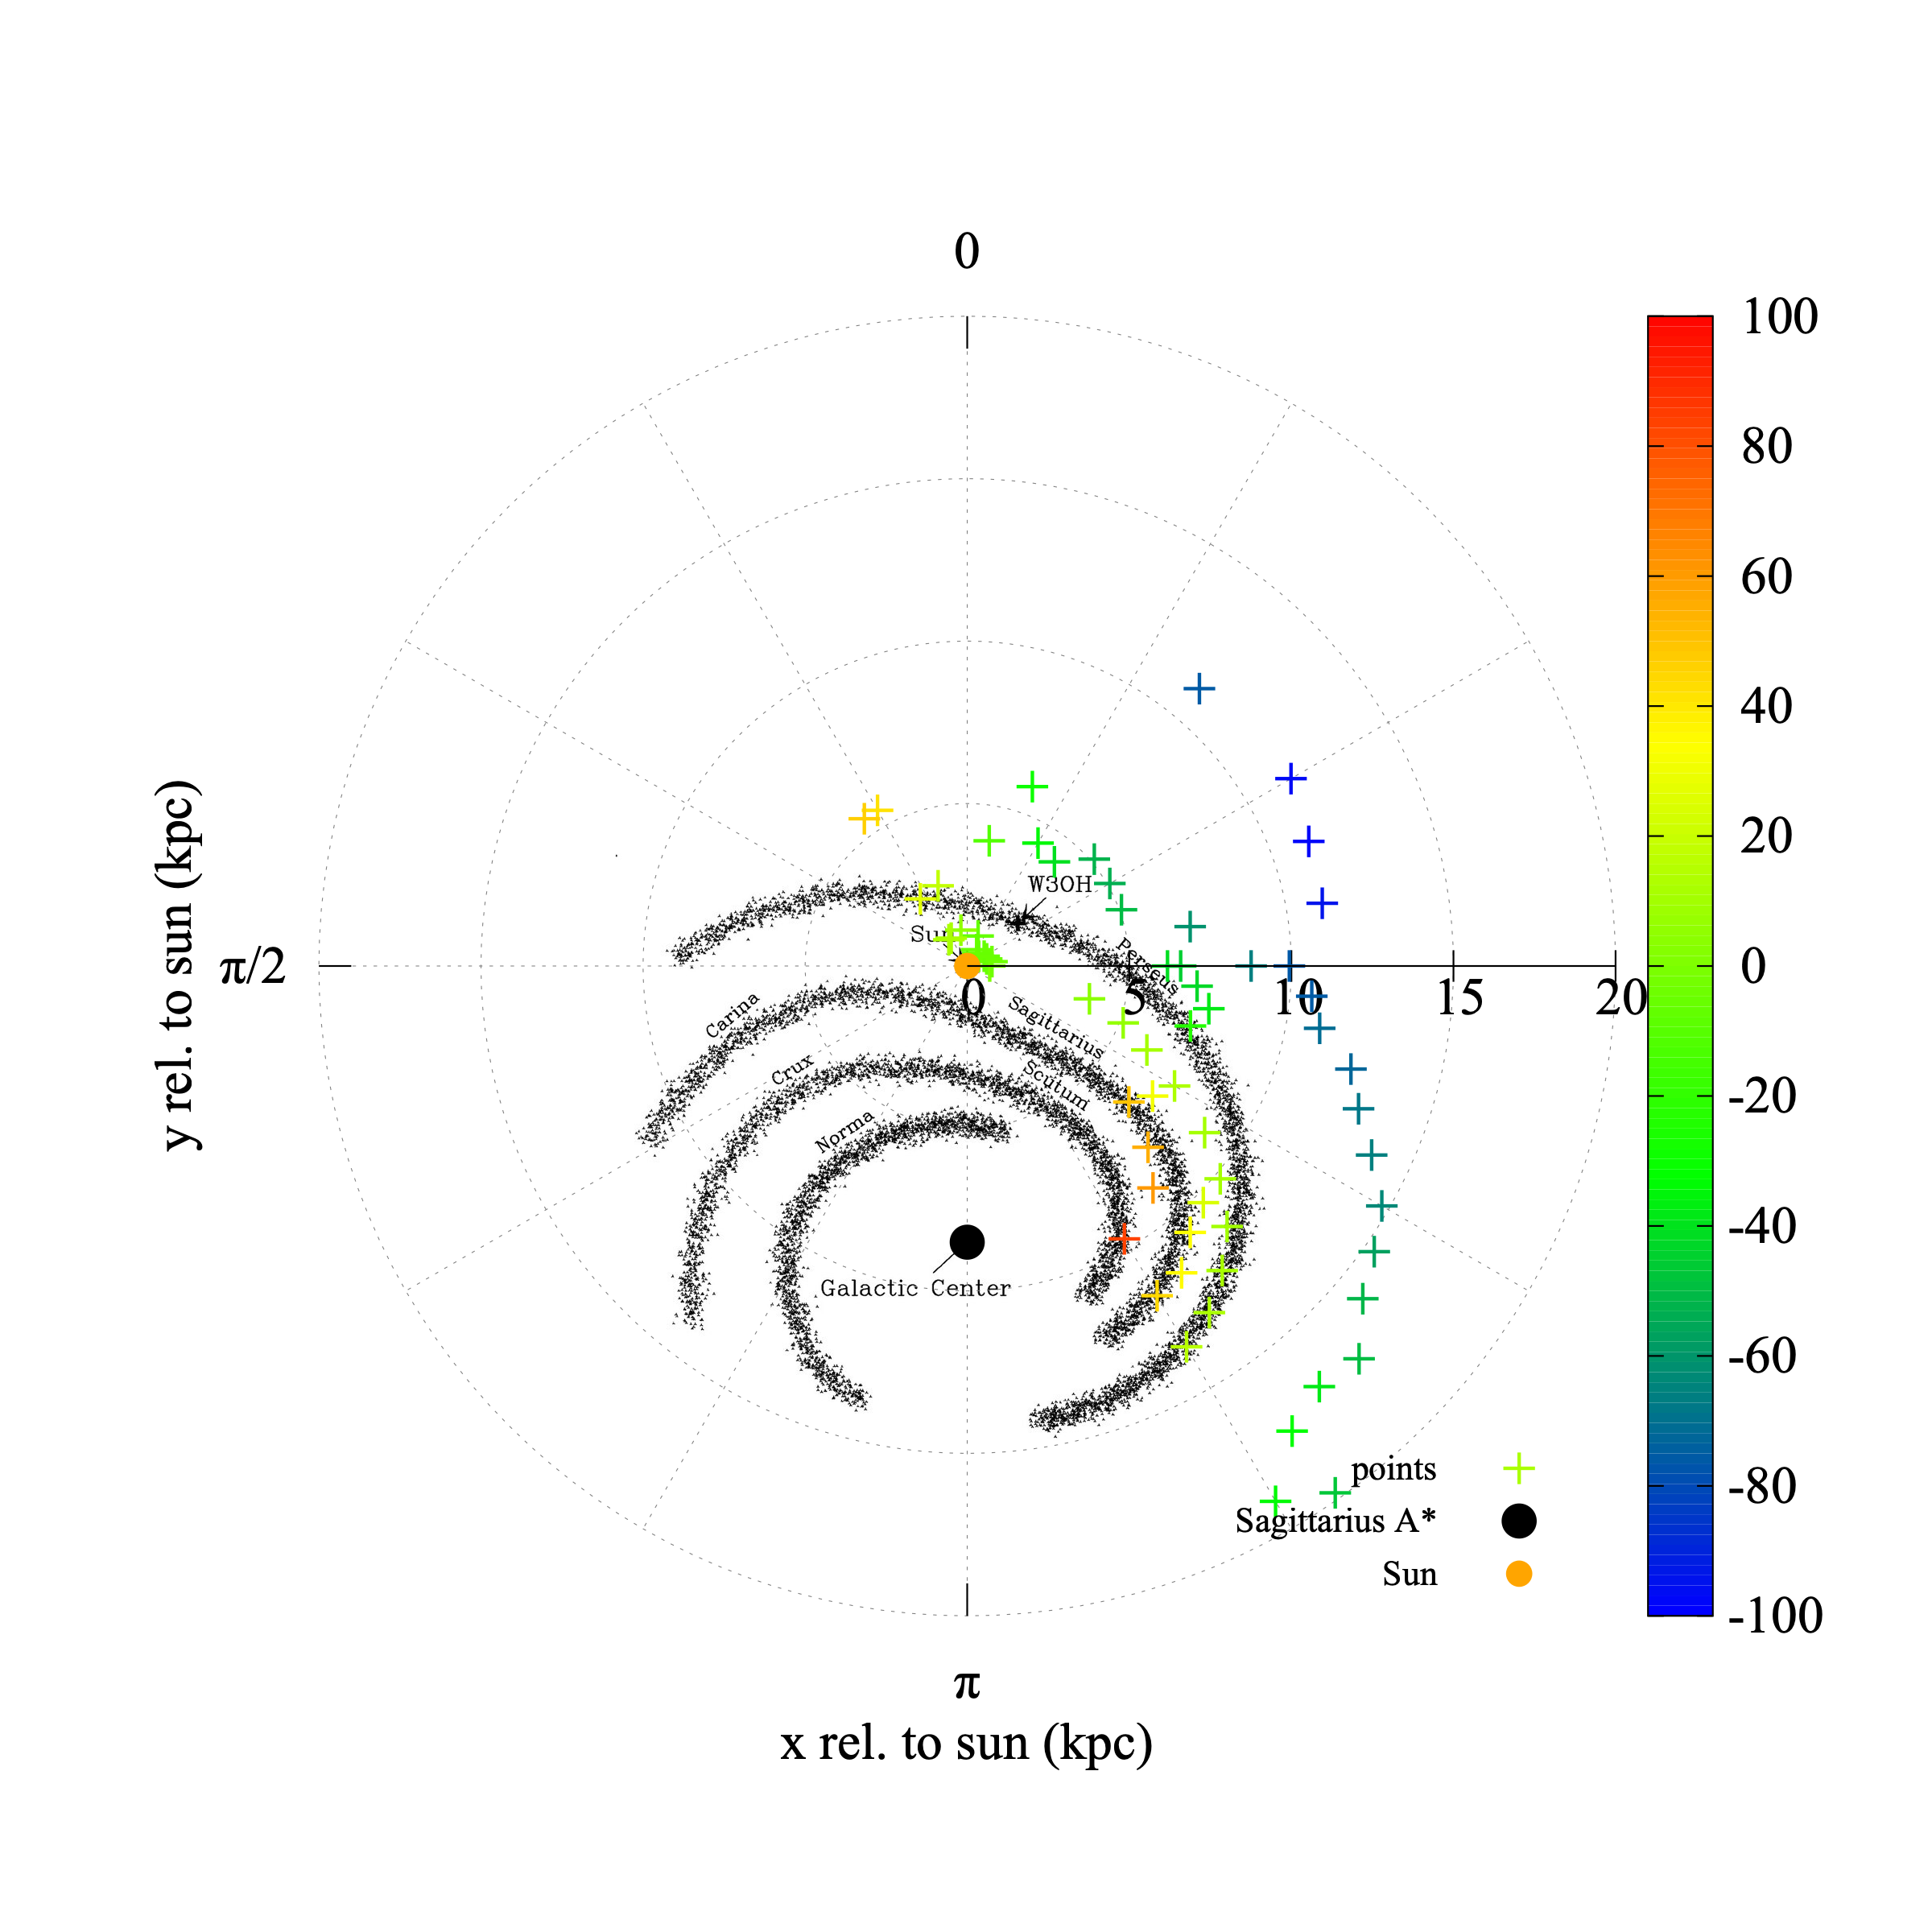
\includegraphics[width=0.8\textwidth]{Bilddateien/MilkyMap/combined_gfx_1.pdf}
        \caption{Überlagerung der Messergebnisse mit einer Karte der Milchstraße aus \cite{doi:10.1126/science.1120914}.}
        \label{fig:combinedMilkyWay}
    \end{figure}
    Gut ersichtlich wird hier die Übereinstimmung der Messpunkte zu den Armen \emph{Scutum}, \emph{Saggitarius} und \emph{Perseus} bei $\SI{210}{\degree}$, welche jedoch Richtung $\SI{270}{\degree}$ weiter zerfließen. Hier werden die Messpunkte zunehmend Beim Perseus Arm erkennbar, teilweise mit großen Abweichungen von der Schematik. 
    
    Für die äußeren Punkte müssen wir eine weitere Grafik herbeiziehen. Anhand dieser werden die Vermischungen bei $\SI{270}{\degree}$ weiter erklärbar: Es könnte sich hier um den \emph{Orion-Cygnus} Arm handeln, welcher die Sonne beinhaltet. Betrachte hierzu Abbildung \ref{fig:ArmSchematikII}.
    \begin{figure}[H]
        \centering
        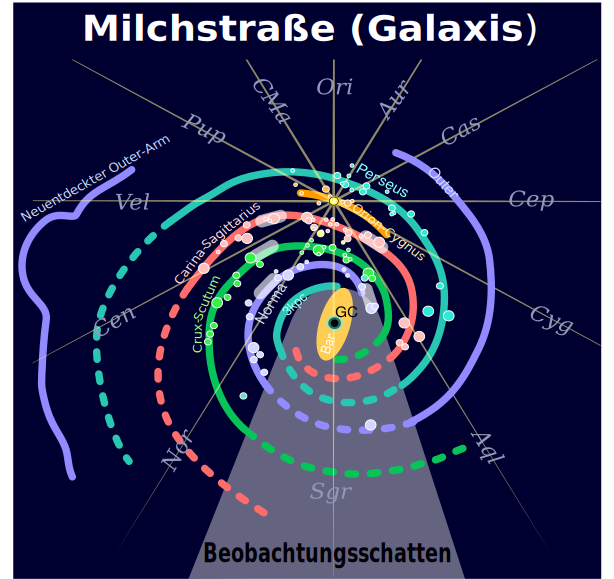
\includegraphics[width=0.8\textwidth]{Bilddateien/MilkyMap/Milky_Way_Arms_de.pdf}
        \caption{Weitere schematische Grafik der Milchstraße aus \cite{wiki:ArmSchematikII}.}
        \label{fig:ArmSchematikII}
    \end{figure}
    Die weiter entfernten Messpunkte in \ref{fig:combinedMilkyWay} könnten sich hier mit den \emph{outer arms}, sowie einem Endstück des \emph{Crux Scutums} in Verbindung bringen lassen. 

    Insgesamt lassen sich Zuordnungen jedoch lediglich schätzen, da auch hier wie bereits oben diskutiert eine detailierte Unsicherheitsanlyse aufgrund des hohen Rechenaufwandes ausbleiben muss. 
\end{document}